\documentclass{article}
\usepackage[utf8]{inputenc}
\usepackage[spanish]{babel}
\usepackage[]{amsthm}
\usepackage{amsmath}
\usepackage[]{amssymb}
\usepackage{graphicx}
\usepackage{wrapfig}
\usepackage[letterpaper, margin=1.5in]{geometry}
\usepackage[hidelinks]{hyperref}
\usepackage{url}
\usepackage{listings}
\decimalpoint


\begin{document}
    \begin{titlepage}
        \begin{center}
            \begin{figure}
                \centering
                
\includegraphics[scale=0.13]{../../../logo_itesm.png}\\ % Logo de la institución
            \end{figure}
        \vspace{5cm}
        \LARGE{Instituto Tecnológico y de Estudios Superiores de Monterrey}\\
        \fontsize{12}{14}\selectfont
        \vspace{1cm}
        \textbf{Actividad 3.1. Crear una red en Packet Tracer}\\ % Nombre de la tarea
        \vspace{0.7cm}
        Juan Pablo Echeagaray González\\ % Nombre de autor 1
        \vspace{0.2cm}
        A00830646\\ % Matrícula autor 1
        \vspace{0.7cm}
        Análisis de Criptografía y Seguridad\\ % Materia
        \vspace{0.2cm}
        MA2003B.300\\ % Clave de la materia
        \vspace{0.2cm}
        Dr. Alberto Francisco Martínez Herrera\\ % Nombre del profesor
        \vspace{0.7cm}
        29 de mayo del 2022\\ % Fecha de entrega
        \end{center}
    \end{titlepage}

    \section{Reporte}

        Para la realización de esta tarea se hizo uso del software \emph{Cisco Packet Tracer} en su versión 8.1.1.0222 en una máquina corriendo \emph{Windows 10} de 64 bits \cite{packet-tracer}. Se comenzó por la implementación de la topología mostrada en la figura \ref{fig:network-topology}. Para este paso no se necesita realizar una configuración de la mayoría de los equipos, a excepción de \emph{Laptop0}, este componente tiene que apagarse para instalarle el adaptador de red inalámbrica \emph{WPC300N}.

        Después se cambió la naturaleza del IP de cada \emph{PC} de estático a seguir el protocolo \emph{DHCP}. Esto se realiza desde la ventana \emph{Config} de cada equipo. Cuando cada máquina tuvo esta configuración, se obtuvo el IP de cada una por medio del comando \lstinline{ipconfig} ejecutado en la terminal de cada una de las máquinas. Los IP correspondientes se presentan en la tabla \ref{table:pc-ips} y una visualización del resultado de ejecutar dicho comando se encuentra en la figura \ref{fig:ipconfig-test}.

        \begin{table}[h!]
            \centering
            \begin{tabular}{ ||c|c|| }
                \hline
                Máquina & IP \\[0.5ex]
                \hline \hline
                PC0 & 169.254.214.147 \\
                \hline
                PC1 & 169.254.13.29 \\
                \hline
                PC2 & 169.254.77.219 \\
                \hline
            \end{tabular}
            \caption{IP asignado a cada máquina}
            \label{table:pc-ips}
        \end{table}

        Una vez que se conocían los IP de cada equipo se utilizó el comando \lstinline{ping XXX.XXX.XXX.XXX} para verificar que existía una conexión entre cada uno de los equipos. Una visualización de la ejecución de este comando se encuentra en la figura \ref{fig:ping-test}.

        Después se trataron los equipos de conexión inalámbrica, se consiguieron los IP asignados a cada uno de estos equipos por el mismo método descrito con anterioridad, un concentrado de los IP se encuentra en la tabla \ref{table:wireless-ips}.

        \begin{table}[h!]
            \centering
            \begin{tabular}{ ||c|c|| }
            \hline
            Máquina & IP \\[0.5ex]
            \hline \hline
            Laptop0 & 192.168.0.103 \\
            \hline
            Tablet PC0 & 192.168.0.100 \\
            \hline
            Smartphone0 & 192.168.0.102 \\
            \hline
            \end{tabular}
            \caption{IP asignado a Laptop, Tablet y Smartphone}
            \label{table:wireless-ips}
        \end{table}
        
        \subsection{Reflexión}
            
            Cuando se simuló esta red los dispositivos inalámbricos se conectaron de forma automática al router \emph{WRT300N}, esto sucede porque no se le asignó una clave al router, para efectos prácticos el router simulado es similar a una red abierta. El efecto de conexión es similar al de nuestros equipos electrónicos para con las redes que tengamos instaladas en nuestros hogares, pero la diferencia es que estos se conectan de forma automática porque ya tienen guardada la clave de conexión al router; para evitar que cualquier dispositivo se conecte al router simulado debemos de asignarle una clave.


    % Bibliografía
    \clearpage
    \bibliographystyle{apalike}
    \bibliography{references.bib}
    
    % Apéndice
    \clearpage
    \appendix

    \section{Figuras}

        % Network topology
        \begin{figure}[h!]
            \centering
            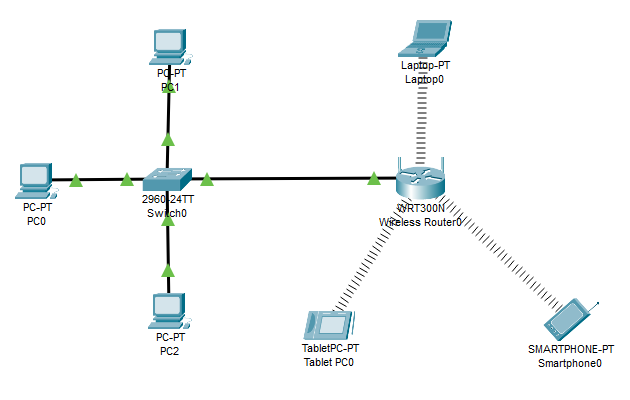
\includegraphics[scale=0.8]{img/network-topology.png}
            \caption{Topología de la red}
            \label{fig:network-topology}
        \end{figure}

        % ipconfig test on PC0
        \begin{figure}[h!]
            \centering
            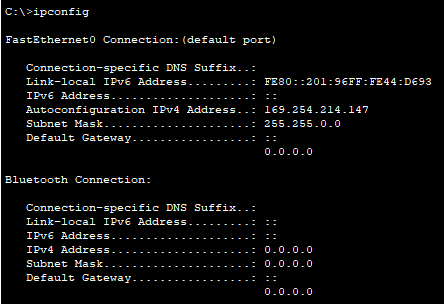
\includegraphics[scale=0.8]{img/ipconfig-test.png}
            \caption{Captura del IP de PC0}
            \label{fig:ipconfig-test}
        \end{figure}

        % Ping test
        \clearpage
        \begin{figure}[h!]
            \centering
            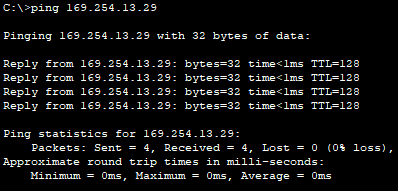
\includegraphics[scale=0.8]{img/ping-test.png}
            \caption{Prueba de conexión entre PC0 y PC1}
            \label{fig:ping-test}
        \end{figure}

\end{document}